\documentclass[tikz]{standalone}

\usepackage{tkz-euclide}
\usepackage{fourier-otf}
\usepackage{fontspec}

\begin{document}
  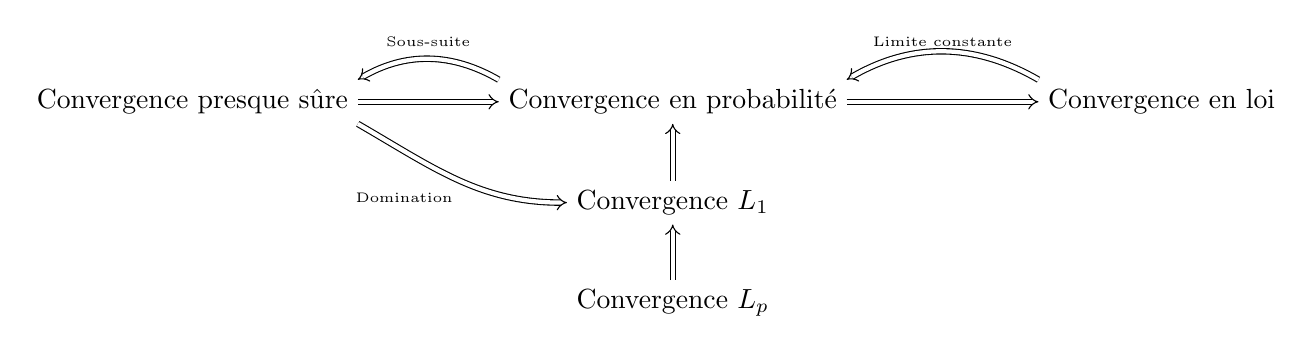
\begin{tikzpicture}
  	\node (A) at (0,0) {Convergence presque sûre};
  	\node (B) at ($(A.east)+(4,0)$) {Convergence en probabilité};
  	\node (C) at ($(B.south)+(0,-1)$) {Convergence $L_1$};
  	\node (D) at ($(B.east)+(4,0)$) {Convergence en loi};
  	\node (E) at ($(C.south)+(0,-1)$) {Convergence $L_p$};
  	\draw[-implies,double equal sign distance] (A) -- (B);
  	\draw[-implies,double equal sign distance] (C) -- (B);
  	\draw[-implies,double equal sign distance] (B) -- (D);
  	\draw[-implies,double equal sign distance] (E) -- (C);
  	\draw[-implies,double equal sign distance] (B.north west) to [out=150,in=30] (A.north east);
  	\node at ($(A.north east)!0.5!(B.north west)+(0,0.3)$) [above] {\tiny Sous-suite};
  	\draw[-implies,double equal sign distance] (D.north west) to [out=150,in=30] (B.north east);
  	\node at ($(B.north east)!0.5!(D.north west)+(0,0.3)$) [above] {\tiny Limite constante};
  	\draw[-implies,double equal sign distance] (A.south east) to [out=-30,in=-180] (C.west);
  	\node at ($(A.south east)!0.5!(C.west)+(0,-0.25)$) [below left] {\tiny Domination};
  \end{tikzpicture}
\end{document}
